\section{Orientation}
$E_N$ depending on the orientation:

\begin{equation}
  E_N = \log_2\left\{
    1 + \abs{
      \sin(
      \frac{G M_A M_B t}{\hbar} \frac{\Delta x_A \Delta x_B}{8L^3}
      \left[ \sin\alpha\sin\beta - \frac{1}{2}\cos\alpha\cos\beta \right]
      )
      }
  \right\}
\end{equation}

Time till the maximum entanglement ($E_N = 1$):
\begin{equation}\label{eq:4:t-max}
  t_\mathrm{max} = \frac{8 \pi L^3 \hbar}{2 G M_A M_B \Delta x_A\Delta x_B} \abs{\sin\alpha\sin\beta - \frac{1}{2}\cos\alpha\cos\beta}^{-1}
\end{equation}

with a global minimum for $\alpha,\beta \in [0, \pi]$ for the orthogonal orientation with $\alpha = \beta = \pi/2$. Here, the time till the maximum entanglement is given by
\begin{equation}
  t_\mathrm{max} = \frac{4 \pi \hbar L^3}{G M_A M_B \Delta x_A \Delta x_B} \simeq 129\si{mn}
\end{equation}

\begin{figure}[!htbp]
  \centering
  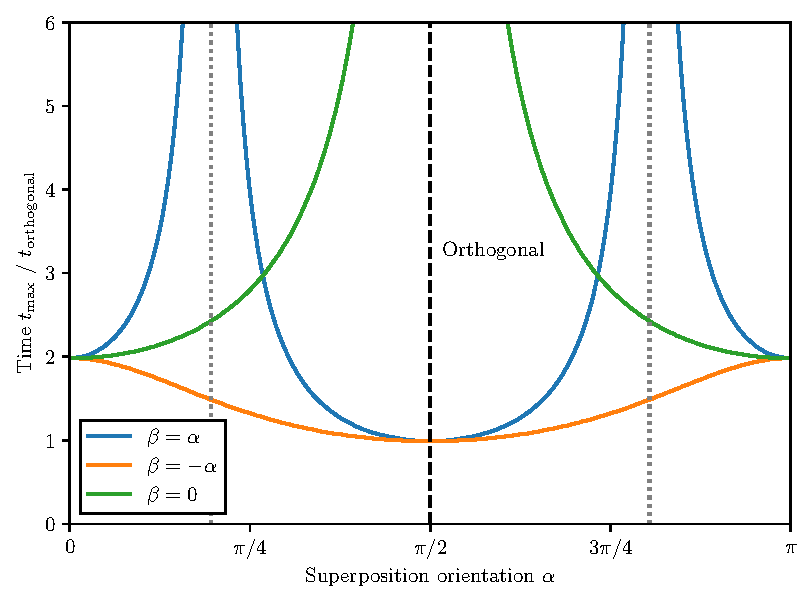
\includegraphics[width=\textwidth]{./../figures/ideal-entanglement/EN-orientation.pdf}
  \caption{Time until maximal entanglement $t_\mathrm{max}$ for different orientations of the angled $\alpha$ and $\beta$ (refer to \cref{fig:4:problem-scetch}). The \textit{parallel configuration} corresponds to $\alpha = \pm\beta = k\pi$ and the \textit{orthogonal configuration} to $\alpha = \pm\beta = k\pi - \pi/2$ ($k \in \mathbb{Z}$). The minimal time is reached for the orthogonal configuration.}
  \label{fig:4:tmax-orientation}
\end{figure}

\begin{figure}[!htbp]
  \centering
  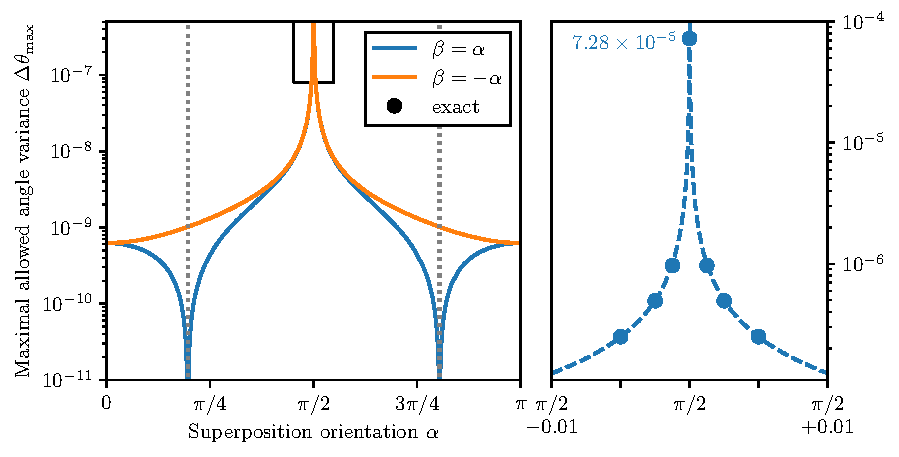
\includegraphics[width=0.95\textwidth]{./../figures/theta-variance/theta-max-orientation-complete.pdf}
  \caption{Maximum possible allowed angular variation $\Delta\theta_\mathrm{max}$ for different orientations. All data-points where calculated at the time of maximum entanglement shown in \cref{fig:4:tmax-orientation}. The \emph{orthogonal configuration} is very stable against angular disturbances. At $\alpha=\beta=\pi/2$, only exact numerical results show a finite value. The singularities on the left figure arise from the fact, that these configurations need infinite time to entangle as already seen in \cref{fig:4:tmax-orientation}.}
  \label{fig:4:theta-max-orientation}
\end{figure}

\begin{figure}[!htbp]
  \centering
  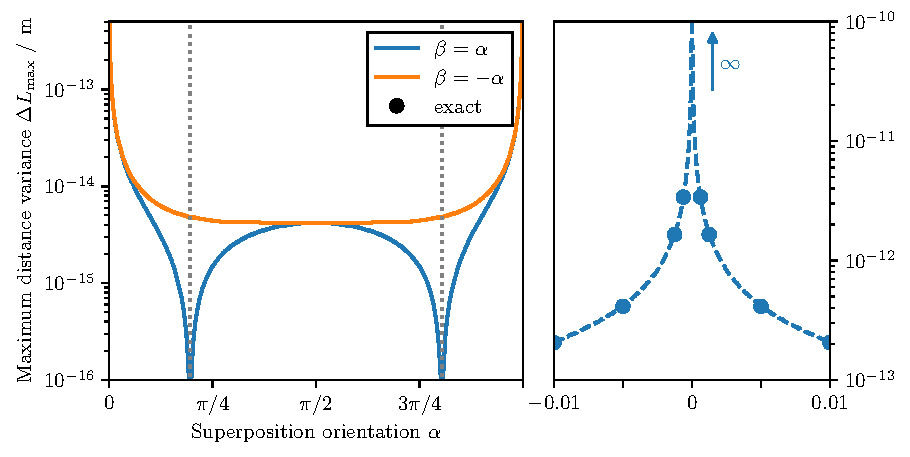
\includegraphics[width=0.95\textwidth]{./../figures/L-variance/L-max-orientation-complete.pdf}
  \caption{Maximum possible allowed distance variation $\Delta L_\mathrm{max}$ for different orientations. This figure is similar to \cref{fig:4:theta-max-orientation}, only for distance variations. On the contrary to angular variations, the \emph{parallel configuration} is infinitely stable against changes in the distance between the shield and the cat-state.}
  \label{fig:4:L-max-orientation}
\end{figure}

\begin{figure}[!htbp]
  \centering
  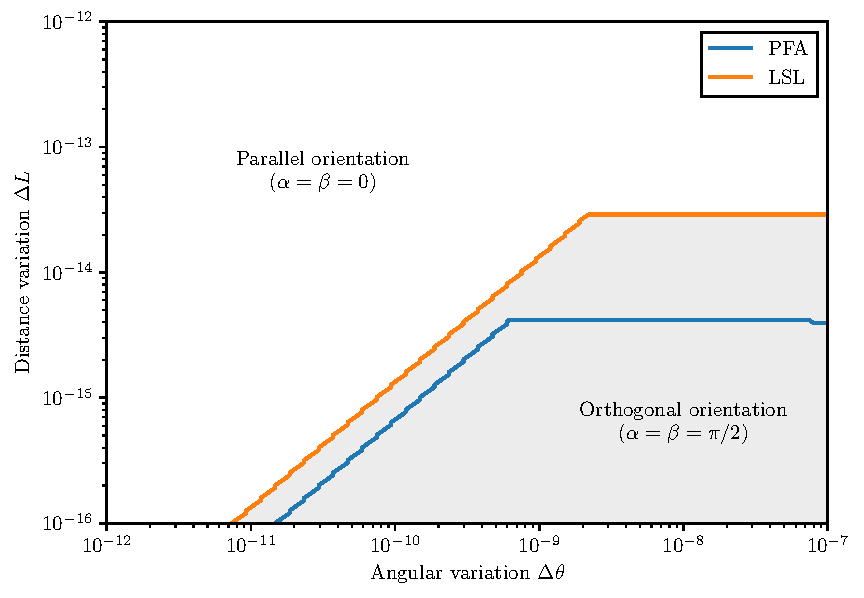
\includegraphics[width=\textwidth]{./../figures/optimize/optimized-orientation.pdf}
  \caption{Optimal orientation for arbitrary variations in the angle $\Delta\theta$ and the distance $\Delta L$. The optimum was calculated for different models of the Casimir-interaction (PFA eq. \eqref{eq:3:casimir-sphere-plate-PFA} and LSL eq. \eqref{eq:3:casimir-sphere-plate-LSL}).If angular variations dominate, the orthogonal configuration is best, whereas for large distance variations, a parallel orientation is advised.}
  \label{fig:4:optimal-orientation}
\end{figure}